\subsection{Automatische Klassifizierung der named entities}
Nachdem man nun die Wahrscheinlichkeit schätzen kann, mit der ein Dokument ``elite'' ist, benötigt man nun noch die Häufigkeit der möglichen Koreferenzen.\\
Dafür müssen wir zunächst herausfinden, von welchem Typ die Entity Query ist. Für Personen wird
\[A_P=\left\{ \text{'he', 'she', 'his', 'her', 'himself', 'herself'} \right\}\]
als sinnvolle Menge von Koreferenzen angesehen. Für Objekte wird eine erweiterbare Menge an Koreferenzen um
\[A_0=\left\{ \text{'it', 'its', \dots} \right\}\]
bei Bedarf verwendet. Das hat den Grund, dass Objekte oft mit Nomen referenziert werden. So wird beispielsweise ``Google'' eventuell mit ``Suchmaschine'', ``Internetriese'' oder ähnlichem bezeichnet.\\
\\
Für die Unterscheidung zwischen Person und Objekt wird ein Support Vector Machine Klassifikator eingesetzt.\\
Dafür werden zunächst Entitäten aus einer Trainingsmenge betrachtet. Bei diesen Eigennamen wird dem Computer als zusätzliche Information mitgeteilt, ob es sich um eine Person oder um ein Objekt handelt. Der Computer versucht dann die besten M Treffer zu den jeweiligen Eigennamen herauszufinden und errechnet charakteristische Werte für diesen Eigennamen. Da wir hier herausbekommen wollen, ob es sich um ein Objekt oder um eine Person handelt, werden bei den Top M Einträgen die Koreferenzen betrachtet. Kommt häufig $A_P=\left\{ \text{'he', 'she', 'his', 'her', 'himself', 'herself'} \right\}$ vor, so wird es wahrscheinlicher, dass es sich die betrachtete Entität eine Person ist. Kommt $A_0=\left\{ \text{'it', 'its'} \right\}$ häufig vor, so handelt es sich wahrscheinlich um ein Objekt. Die Quantifizierung erfolgt normiert nach:
\[f_P\left( Q \right)=\frac{1}{|F\left( Q \right)|}\sum_{d\in F\left( Q \right)} \frac{tf\left( A_P;d \right)}{len \left( d \right)}\]
\[f_O\left( Q \right)=\frac{1}{|F\left( Q \right)|}\sum_{d\in F\left( Q \right)} \frac{tf\left( A_O;d \right)}{len \left( d \right)}\]
Dabei stellt $F\left( Q \right)$ die Menge der besten M Treffer dar, $|F\left( Q \right)|$ die Kardinalität dieser Menge, $tf\left( A_P;d \right)$ die Häufigkeit der Koreferenzen auf Personen in dem jeweiligen Dokument und $len\left( d \right)$ gibt die Anzahl der Worte eines Dokumentes aus.\\
\\
Der Computer errechnet $f_O\left( Q \right)\text{ und } f_P\left( Q \right)$ für jeden Eigennamen der Trainingsmenge. Visualisiert könnte ein Diagramm dazu wie folgt aussehen:
\begin{figure}[h]
	\centering
	\begin{tabular}{c}
		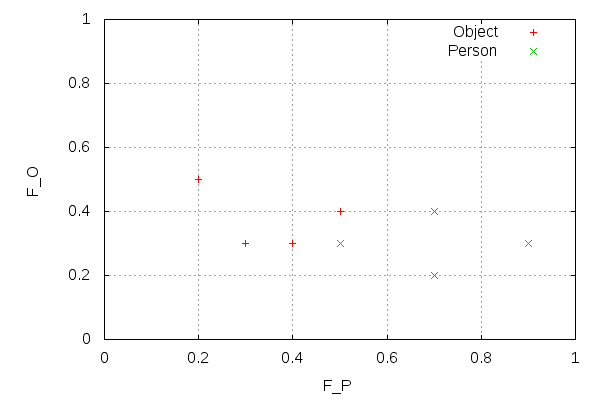
\includegraphics[scale=0.5]{pics/svm_training}
	\end{tabular}
	\caption{Mögliche Visualisierung der SVM nach dem Trainingsschritt ohne Hyperebene}
	\label{tab:svm_training}
\end{figure}\\
Nachdem sich die Eigenschaften von Personen und Objekten hoffentlich etwas unterscheiden und die verschiedenen Typen im Diagramm getrennt erscheinen, muss man nun noch eine Hyperebene mit möglichst großem Abstand zum Rand zwischen den aufgetrennten Typen einfügen. Dafür wurde im Paper über ``A 2-Poisson Model for Probabilistic Coreference of Named Entities for Improved Text Retrieval'' \cite{paper:Na} eine Radial Basis Function herangezogen. 
